%!TEX root = ../thesis.tex
This section will focus on describing and discussing a selection of concepts for ad hoc interfaces based the jamming technique.
As mentioned in the beginning of this chapter we were not succesfull at implementing a working jamming system where we could control air/liquid flow. \todo{make sure this is actually adressed. Suggestions: complexity, price of equipment: mechanics is one thing, the other is materials, i.e. ecoflex rubber etc.}
Therefore we concentrate on conceptual prototypes which we envisioned before taking the descision to move in other directions.

\subsection{(Car) dashboard} 

\todo{what's the problem with static (car) dashboards}\\

Cell-based jamming as mentioned in \ref{ch:jamming} allows for deformations of individual cells.
This technique \hl{opens up} for a new and very dynamic approach to inputs, such as buttons, knobs, etc.
These input controls could emerge from the otherwise flat surface when needed, see figure~\ref{fig:ch:jamming:concepts:button}.
Other than being able to hide input controls when not needed this approach also opens up for a configurable interface adapted to specific users preference.

\begin{figure}[h]
  \centering
      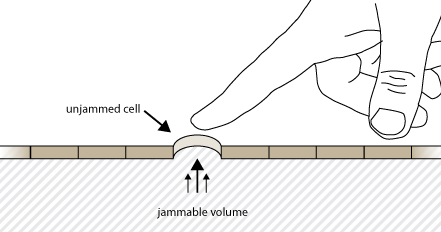
\includegraphics[width=3in]{figures/jamming/concepts/button}
  \caption[A cell-based jammable button.]
  {A cell-based jammable button.}
  \label{fig:ch:jamming:concepts:button}
\end{figure}


